% Source: graduate-coursework/Sp26/CSCE763/Course_Assignments/Project/project_proposal.tex
% Description: YOLOv11-OBB architecture with SAHI tiled inference. Full PPI scans are tiled before single-pass detection, then merged via NMS.

\documentclass[border=4pt]{standalone}
\usepackage{amsmath}
\usepackage{amssymb}
\usepackage{graphicx}
\usepackage{tikz}
\usepackage{xcolor}
\usetikzlibrary{positioning, arrows.meta, calc, fit, backgrounds, decorations.pathreplacing}

\definecolor{USC_Garnet}{HTML}{73000A}
\definecolor{USC_Black10}{HTML}{ECECEC}
\definecolor{USC_Black70}{HTML}{5C5C5C}
\definecolor{USC_Congaree}{HTML}{1F414D}

\begin{document}
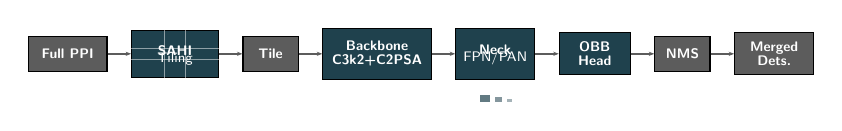
\begin{tikzpicture}[
  scale=0.72, every node/.style={font=\sffamily\tiny},
  block/.style={draw, fill=USC_Congaree, text=white, minimum height=0.45cm,
    minimum width=0.9cm, font=\sffamily\tiny\bfseries, align=center},
  nblock/.style={draw, fill=USC_Black70, text=white, minimum height=0.45cm,
    minimum width=0.9cm, font=\sffamily\tiny\bfseries, align=center},
  arr/.style={-{Stealth[length=2pt]}, thick, USC_Black70}
]
  % Full PPI image
  \node[nblock, minimum width=1.0cm] (ppi) {Full PPI};

  % SAHI Tiling block with grid overlay
  \node[block, right=0.3cm of ppi, minimum width=1.1cm, minimum height=0.6cm] (sahi) {};
  \node[font=\sffamily\tiny\bfseries, white] at ([yshift=0.05cm]sahi.center) {SAHI};
  \node[font=\sffamily\tiny, white] at ([yshift=-0.1cm]sahi.center) {Tiling};
  % Grid overlay lines inside SAHI block
  \draw[white, thin, opacity=0.5] ([xshift=-0.18cm]sahi.south) -- ([xshift=-0.18cm]sahi.north);
  \draw[white, thin, opacity=0.5] ([xshift=0.18cm]sahi.south) -- ([xshift=0.18cm]sahi.north);
  \draw[white, thin, opacity=0.5] ([yshift=-0.1cm]sahi.west) -- ([yshift=-0.1cm]sahi.east);
  \draw[white, thin, opacity=0.5] ([yshift=0.1cm]sahi.west) -- ([yshift=0.1cm]sahi.east);

  % Tile
  \node[nblock, right=0.3cm of sahi, minimum width=0.7cm] (tile) {Tile};

  % Backbone
  \node[block, right=0.3cm of tile, minimum width=1.1cm, minimum height=0.65cm] (back)
    {Backbone\\[-1pt]C3k2+C2PSA};

  % Neck with multi-scale feature visualization
  \node[block, right=0.3cm of back, minimum width=1.0cm, minimum height=0.65cm] (neck) {};
  \node[font=\sffamily\tiny\bfseries, white] at ([yshift=0.08cm]neck.center) {Neck};
  \node[font=\sffamily\tiny, white] at ([yshift=-0.08cm]neck.center) {FPN/PAN};
  % Multi-scale feature map indicators below neck
  \fill[USC_Congaree!70, draw=white, thin]
    ([yshift=-0.4cm, xshift=-0.28cm]neck.south) rectangle ++(0.2cm,0.14cm);
  \fill[USC_Congaree!55, draw=white, thin]
    ([yshift=-0.4cm, xshift=-0.02cm]neck.south) rectangle ++(0.15cm,0.11cm);
  \fill[USC_Congaree!40, draw=white, thin]
    ([yshift=-0.4cm, xshift=0.2cm]neck.south) rectangle ++(0.1cm,0.08cm);

  % OBB Head
  \node[block, right=0.3cm of neck, minimum width=0.9cm] (head) {OBB\\[-1pt]Head};

  % NMS
  \node[nblock, right=0.3cm of head, minimum width=0.7cm] (nms) {NMS};

  % Merged Detections
  \node[nblock, right=0.3cm of nms, minimum width=1.0cm] (out) {Merged\\[-1pt]Dets.};

  % Arrows
  \draw[arr] (ppi) -- (sahi);
  \draw[arr] (sahi) -- (tile);
  \draw[arr] (tile) -- (back);
  \draw[arr] (back) -- (neck);
  \draw[arr] (neck) -- (head);
  \draw[arr] (head) -- (nms);
  \draw[arr] (nms) -- (out);
\end{tikzpicture}
\end{document}
